\subsection{Lab10: Receptor FM estereofónico}
%*********************
\begin{frame}{}

\pgfdeclareimage[width=\paperwidth,height=\paperheight]{bg}{imagenes/fondo_lab}
\setbeamertemplate{background}{\pgfuseimage{bg}}

\bfseries{\textrm{\LARGE Lab10\\ \Large Receptor FM estereofónico}}
\raggedright
\end{frame}
%*********************

\begin{frame}{Receptor FM estereofónico}

\pgfdeclareimage[width=\paperwidth,height=\paperheight]{bg}{imagenes/fondo3}
\setbeamertemplate{background}{\pgfuseimage{bg}}

\begin{figure}[H]
\centering
\vspace{-3mm}
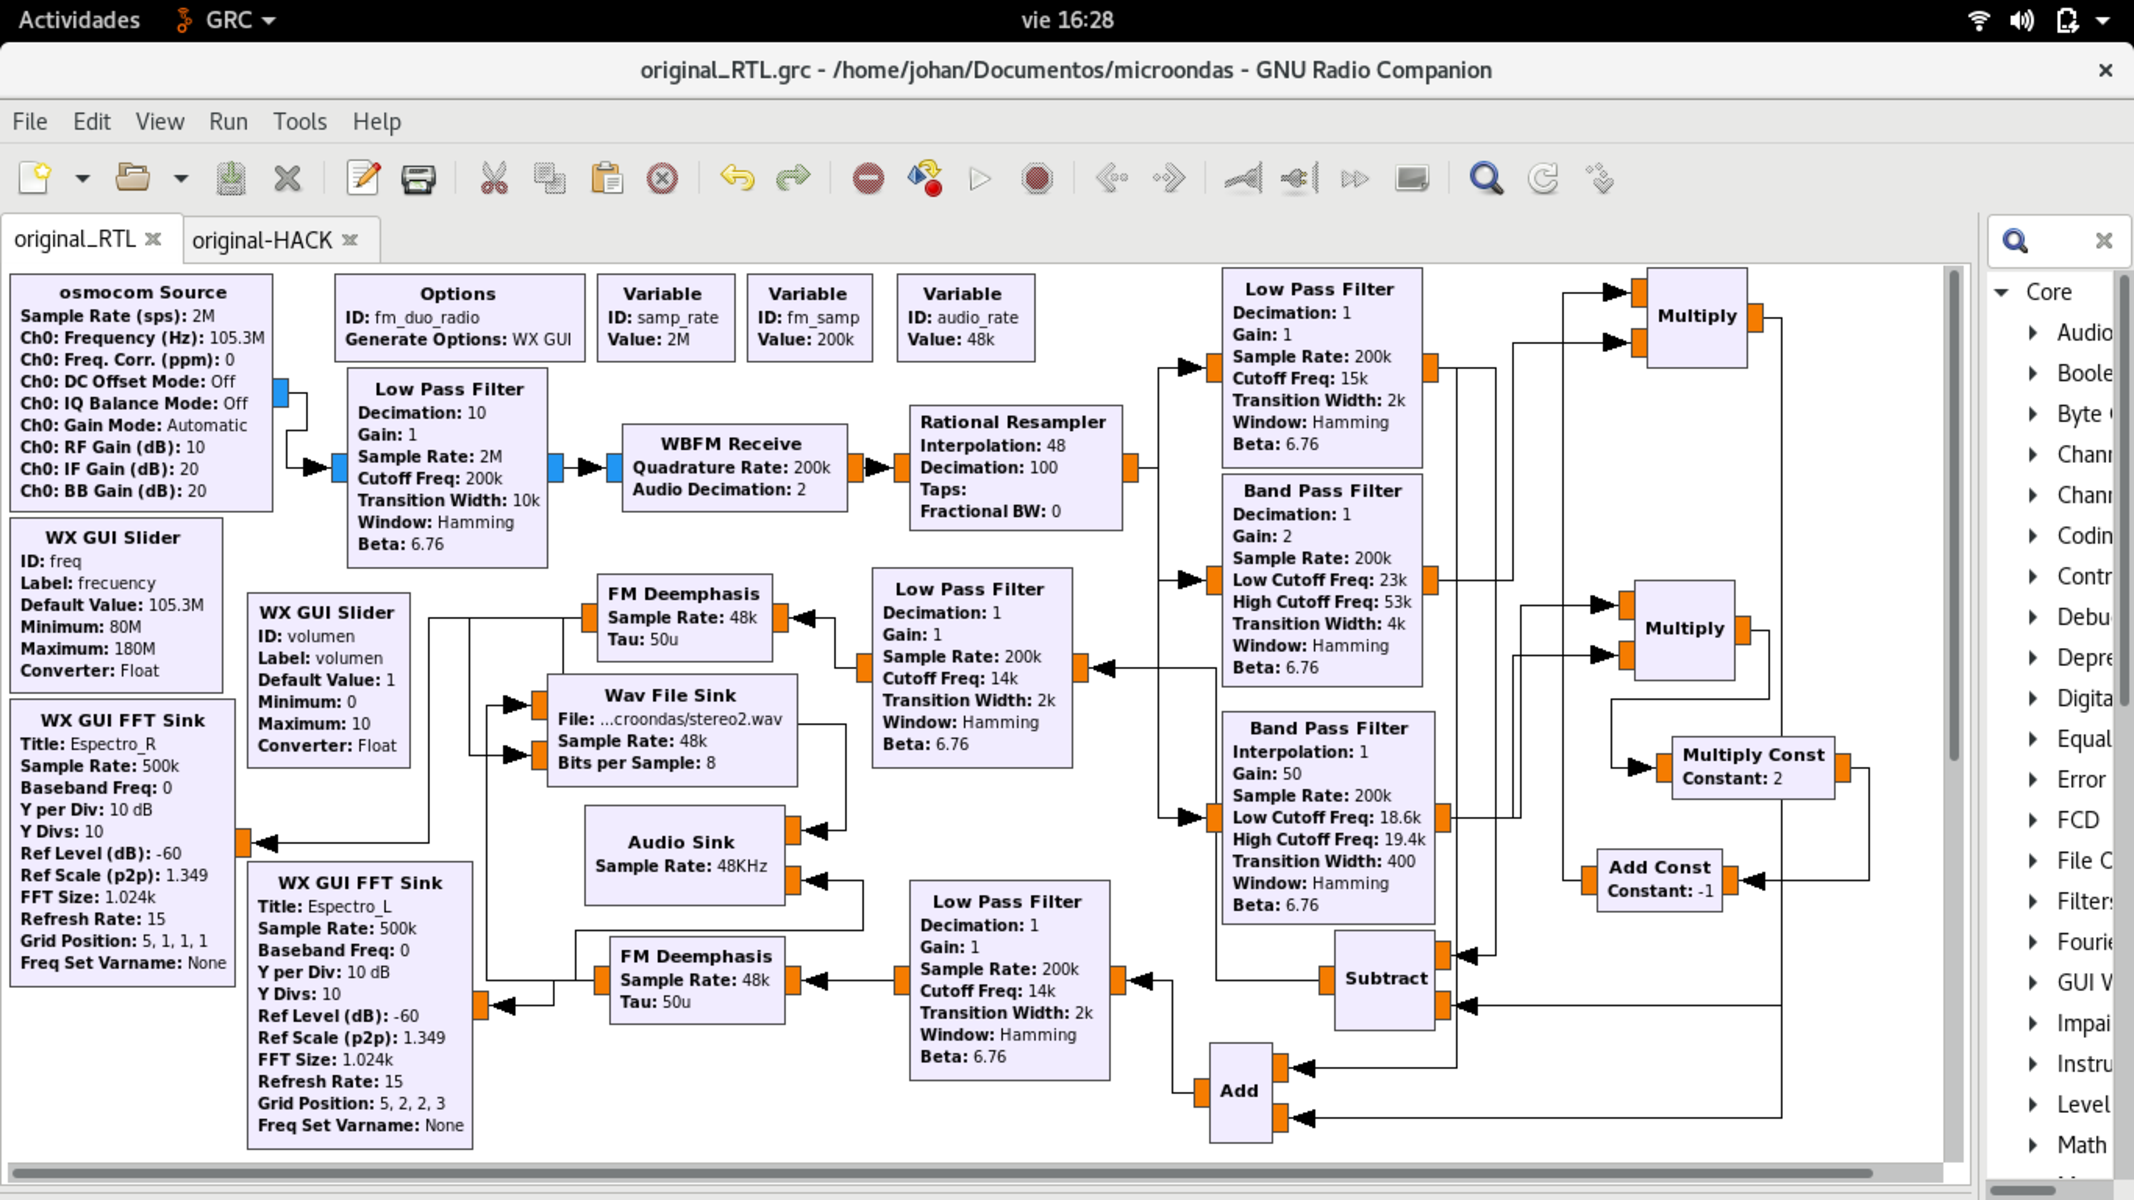
\includegraphics[width=\textwidth]{parte3/lab9/pdf/lab9_1.pdf}
\end{figure}

\end{frame}
%---------------------------------

\begin{frame}{Receptor FM estereofónico}

\begin{itemize}
    \item {La FM, vino a cambiar en todo el esquema que existía en lo que a transmisión y recepción de radio se refiere.}
    \item {Una de las ventajas de FM estéreo es que la reproducción del sonido es tan buena en los receptores estereofónicos como en los de FM normal, estos lo reproducen como una señal monofónica de FM.}
\end{itemize}

\end{frame}
%---------------------------------

\begin{frame}{Receptor FM estereofónico}

\begin{figure}[H]
\centering
\vspace{-3mm}
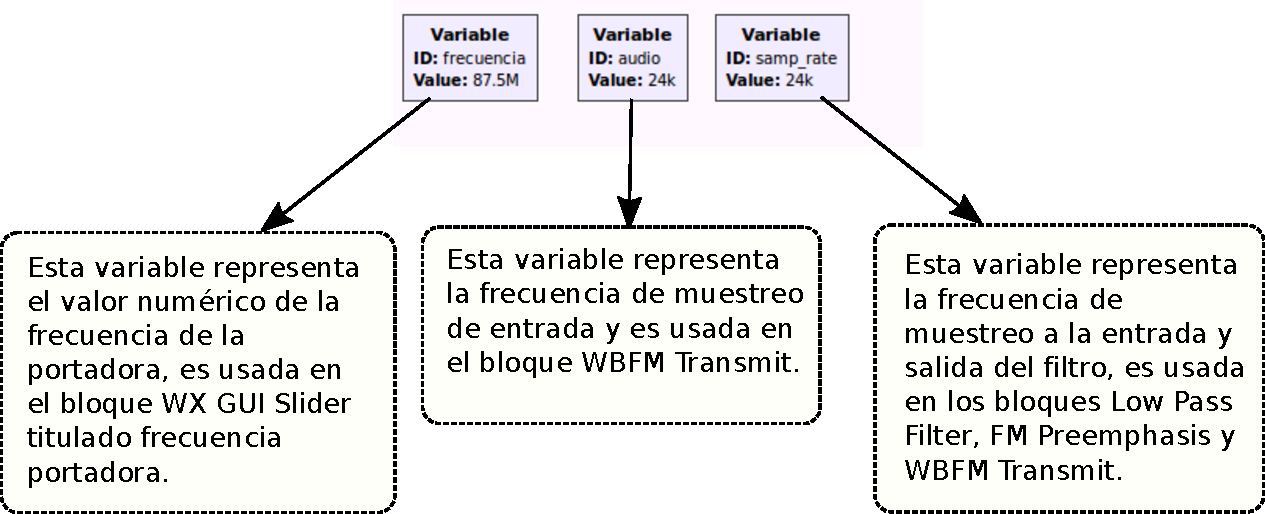
\includegraphics[width=\textwidth]{parte3/lab9/pdf/lab9_2.pdf}
\end{figure}

\end{frame}
%---------------------------------

\begin{frame}{Receptor FM estereofónico}

\begin{figure}[H]
\centering
\vspace{-3mm}
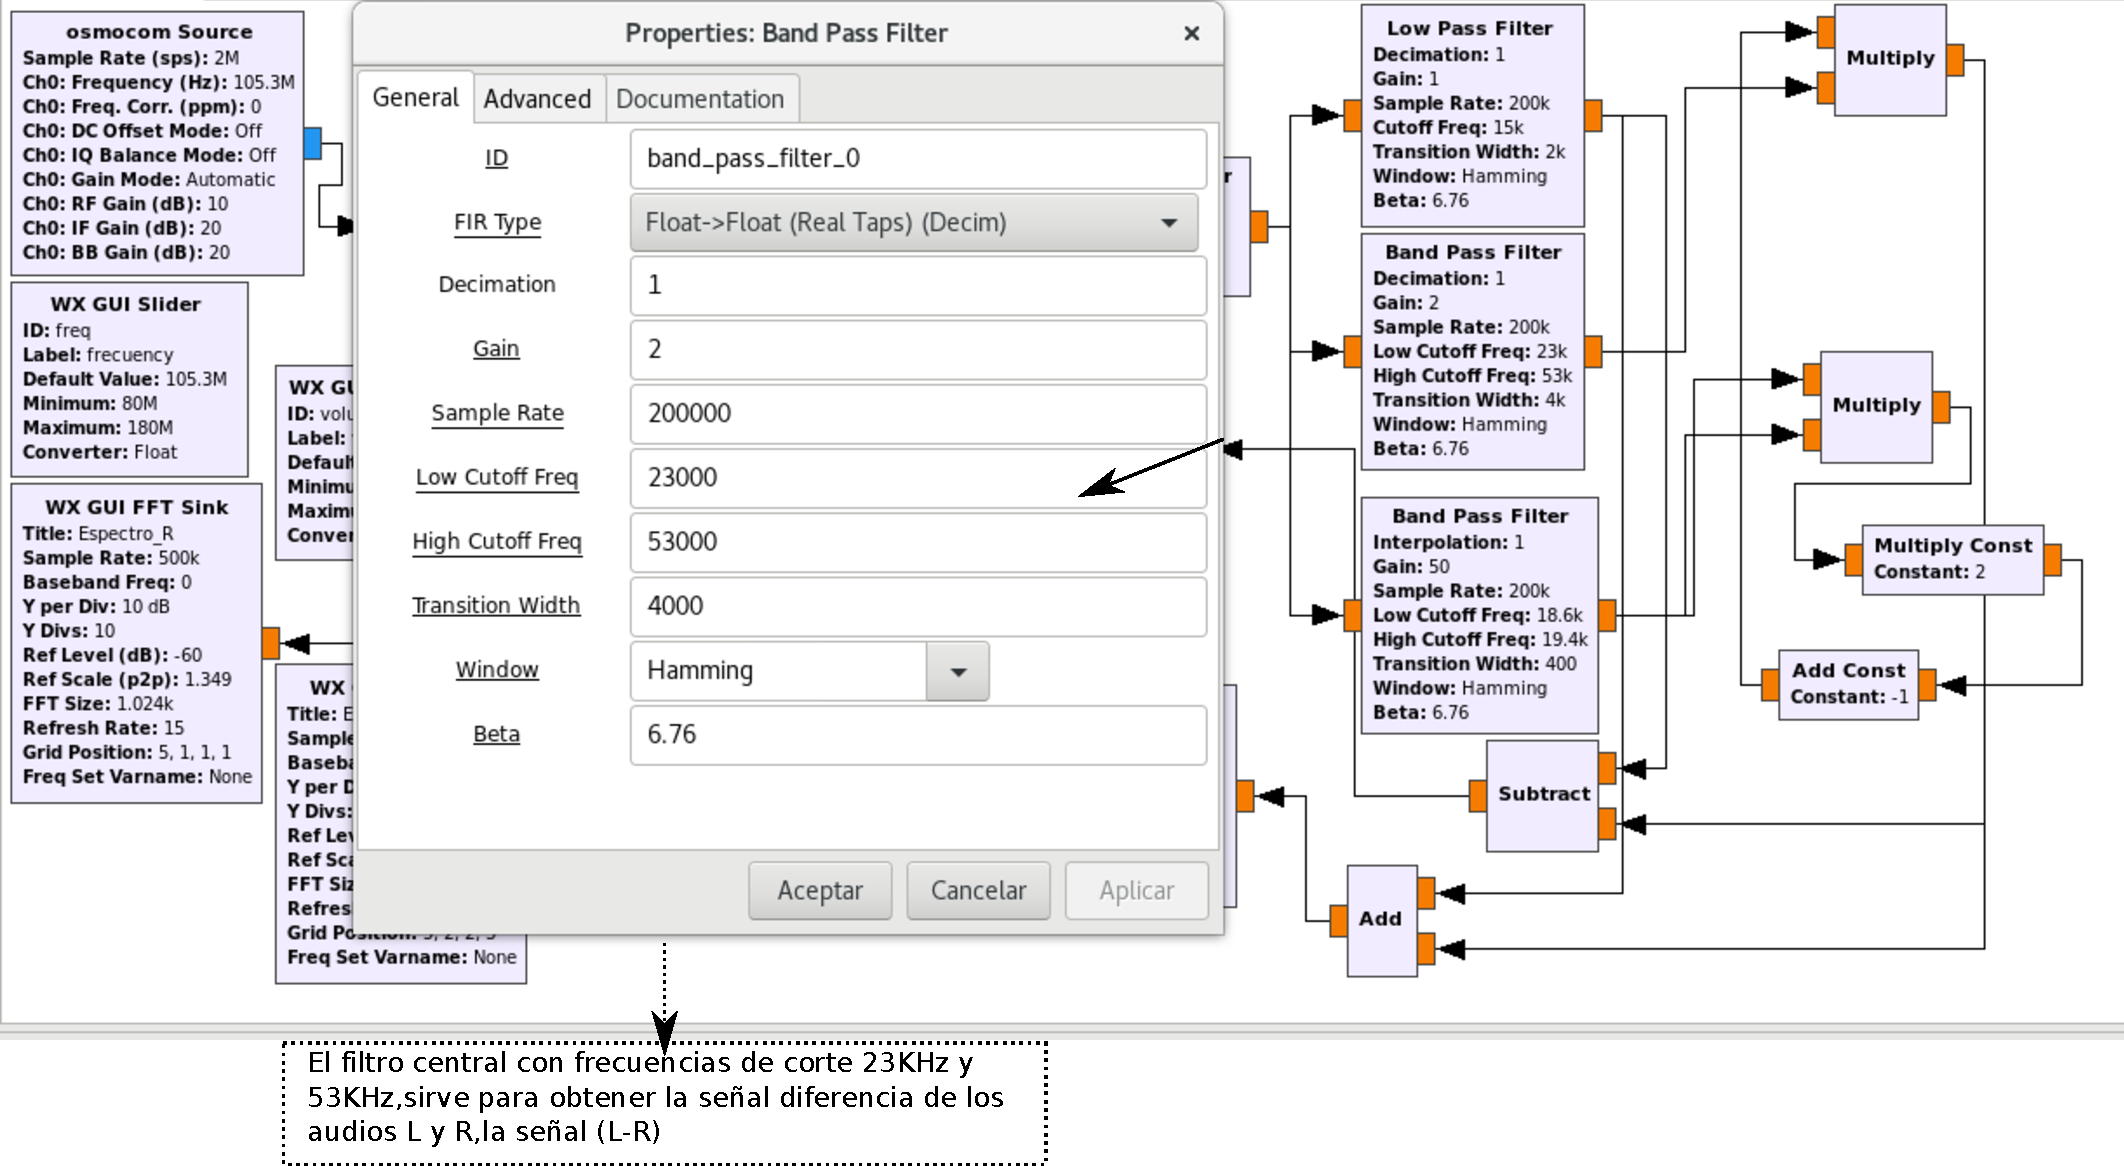
\includegraphics[width=\textwidth]{parte3/lab9/pdf/lab9_3.pdf}
\end{figure}

\end{frame}
%---------------------------------

\begin{frame}{Receptor FM estereofónico}

\begin{figure}[H]
\centering
\vspace{-3mm}
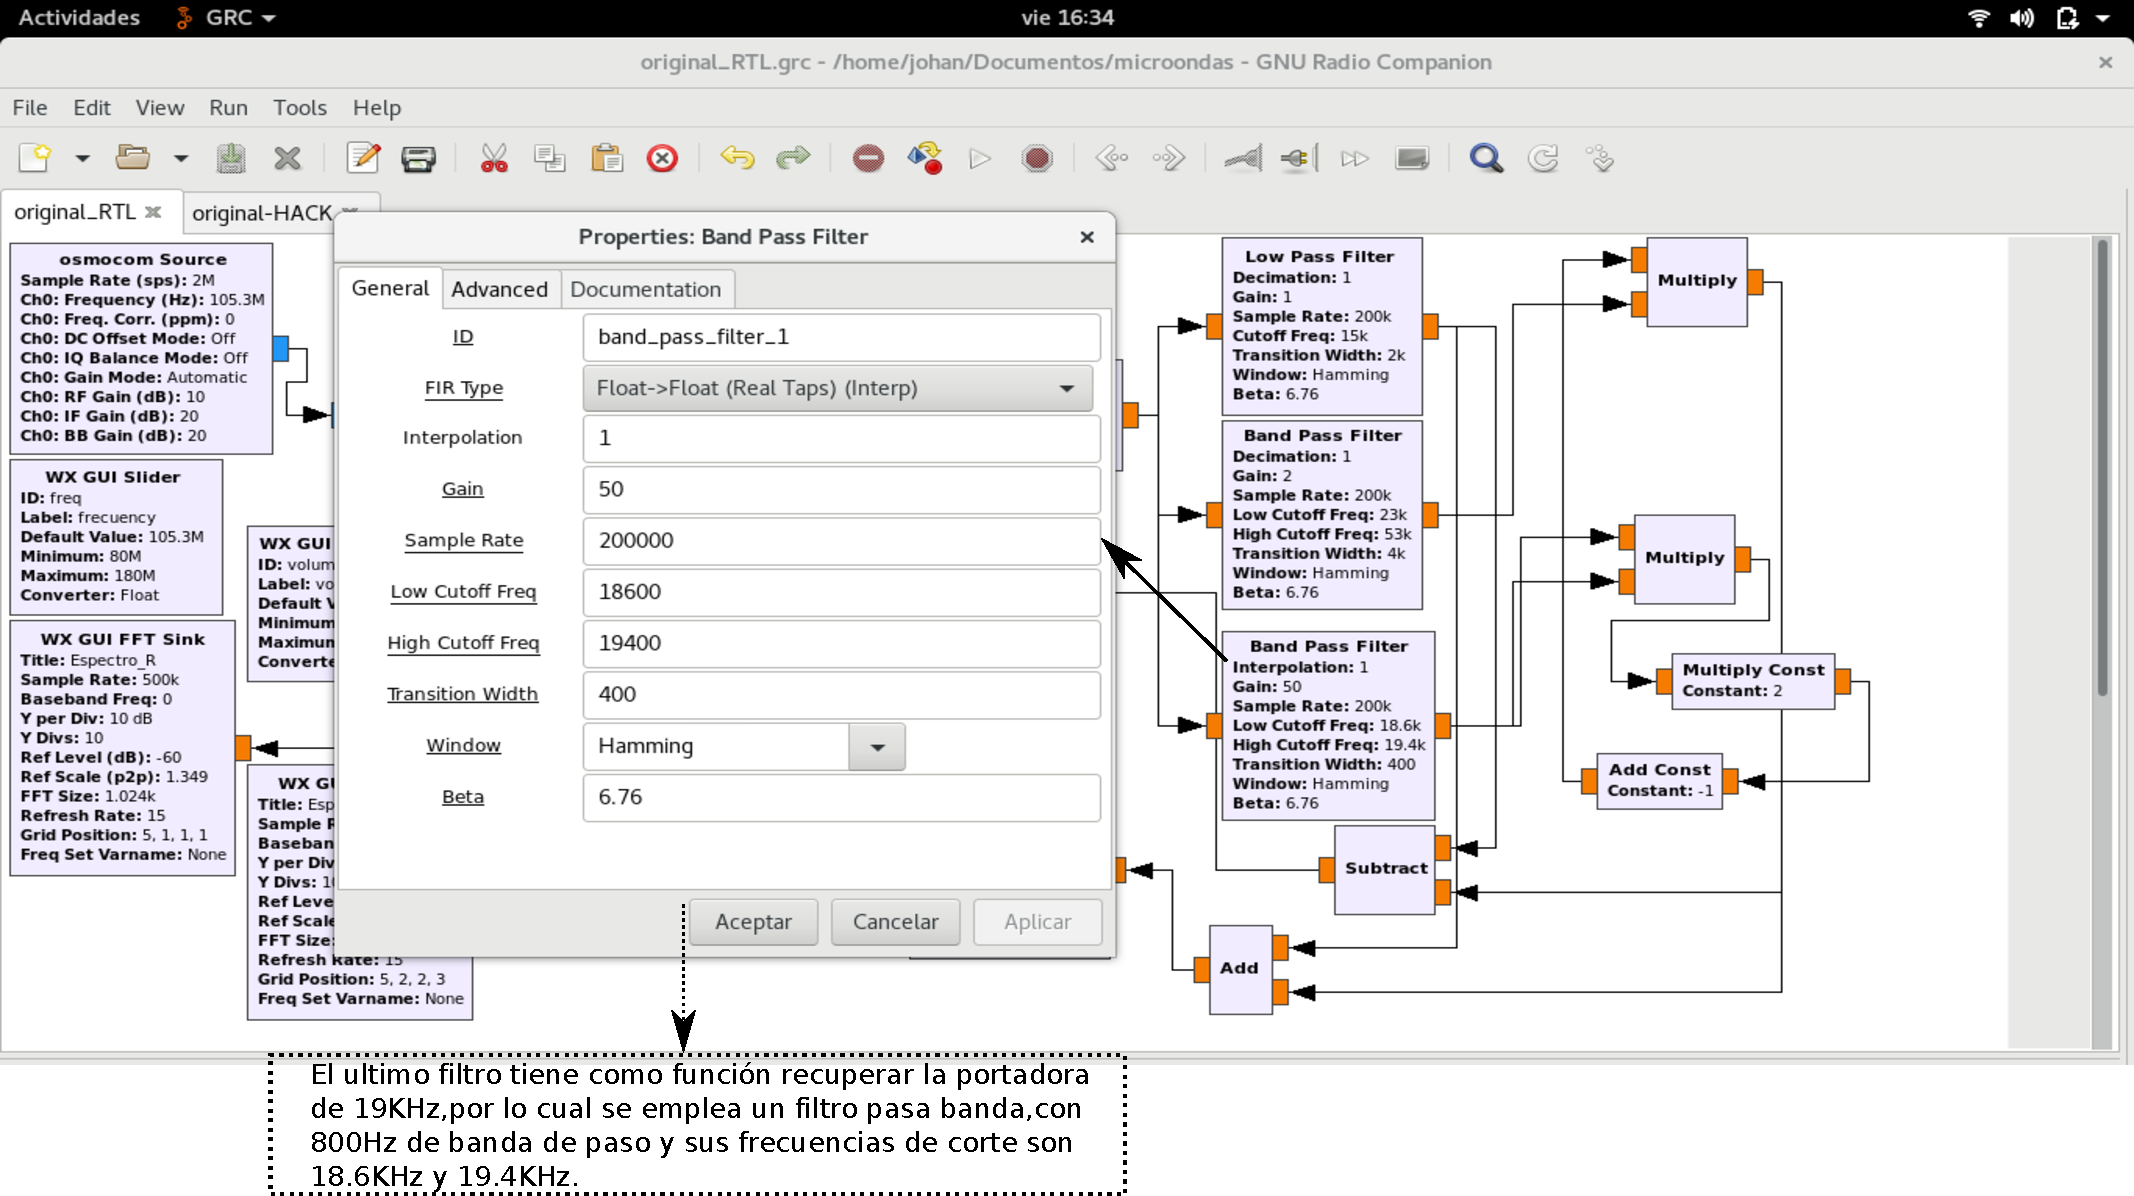
\includegraphics[width=\textwidth]{parte3/lab9/pdf/lab9_4.pdf}
\end{figure}

\end{frame}
%---------------------------------

\begin{frame}{Receptor FM estereofónico}

\begin{figure}[H]
\centering
\vspace{-3mm}
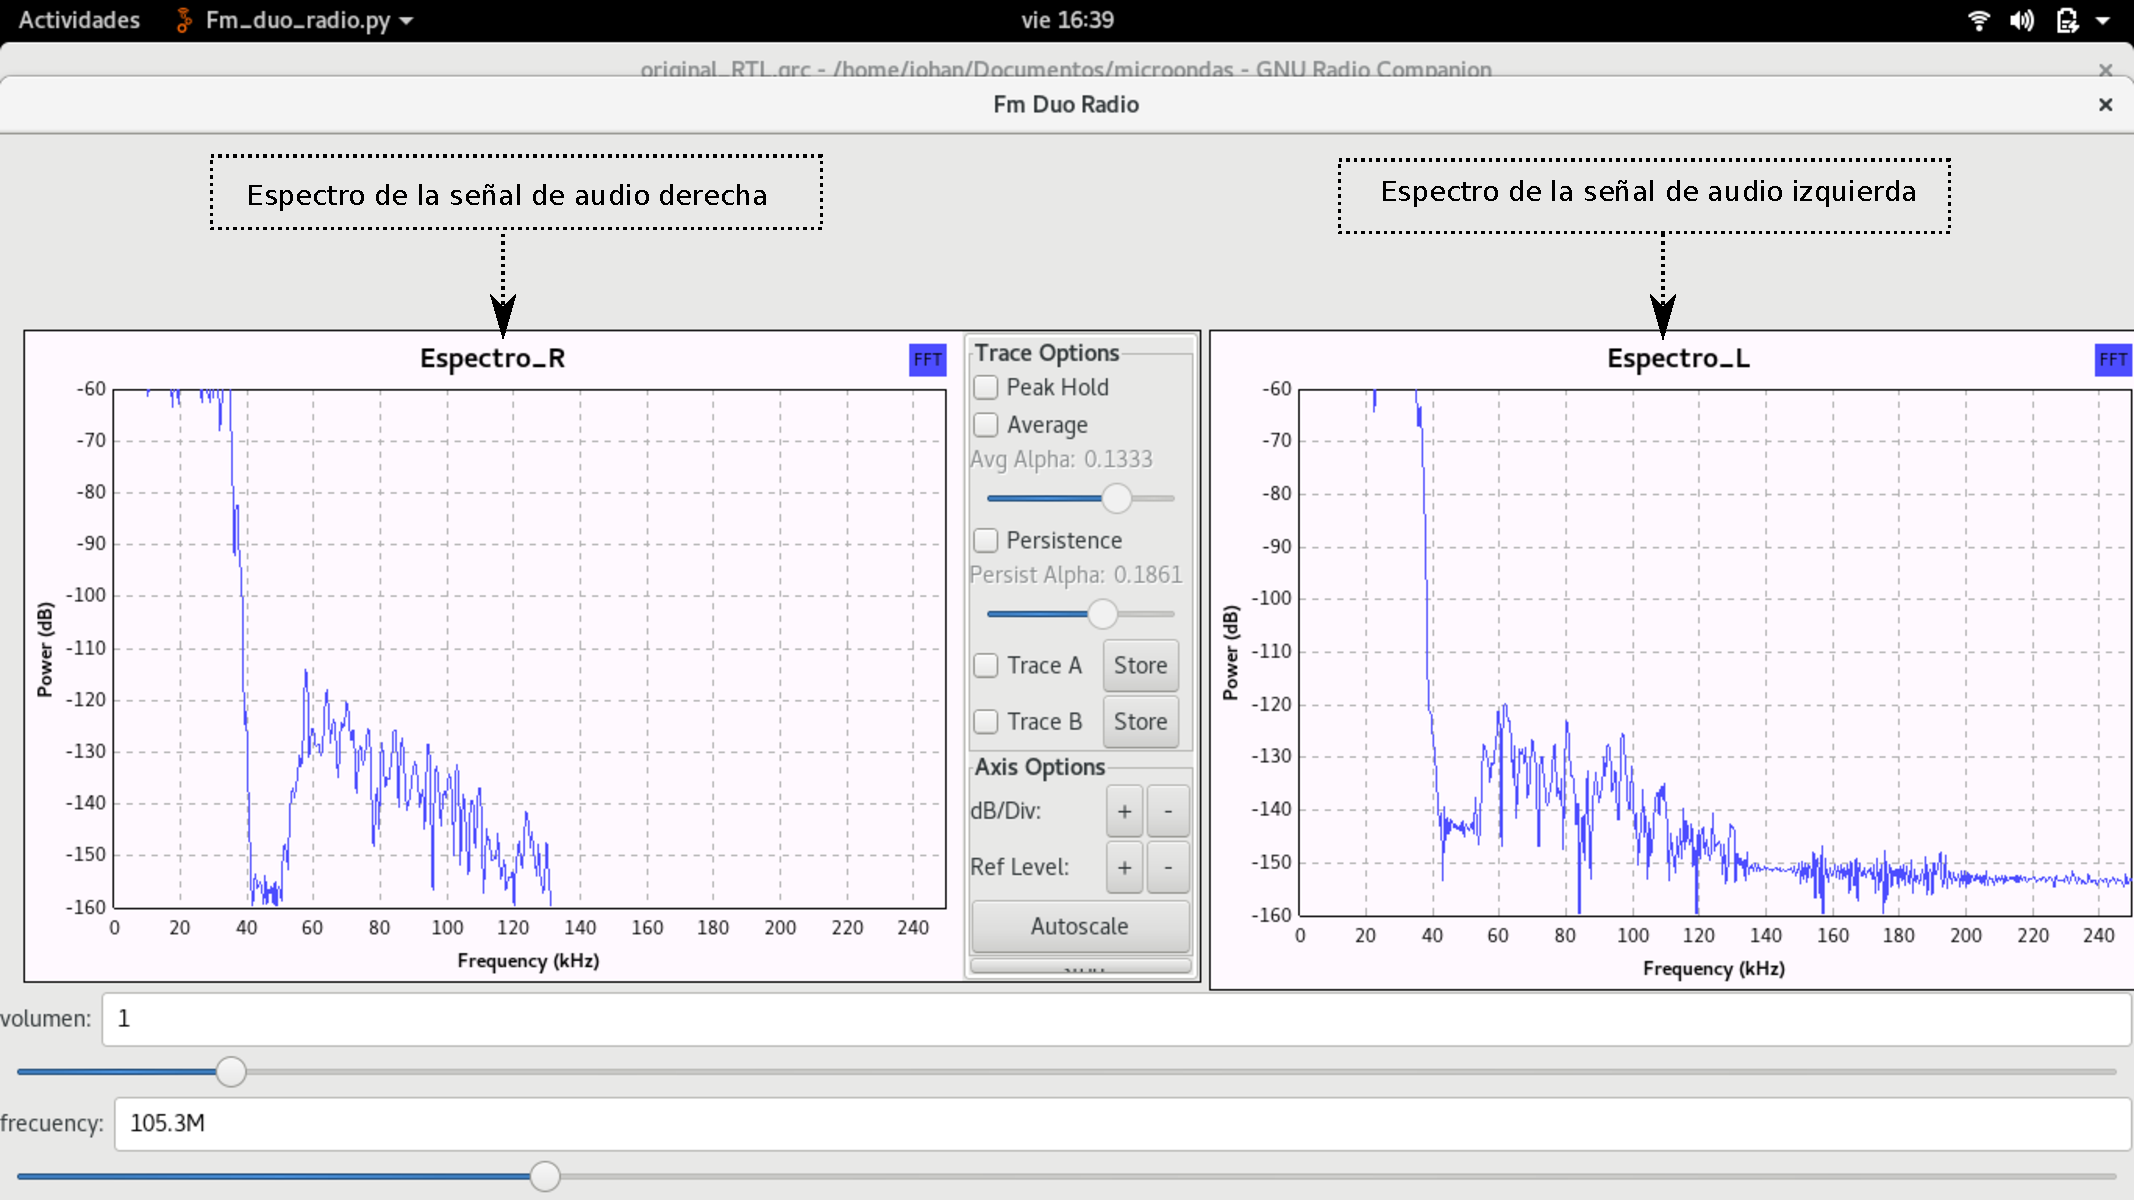
\includegraphics[width=\textwidth]{parte3/lab9/pdf/lab9_5.pdf}
\end{figure}

\end{frame}
%---------------------------------
